% Lecture 11 - 2024-02-02
\section{Function of several variables}
\begin{definition}\quad 
\begin{itemize}
    \item[(a)] A function of two variables is a rule that assigns to each ordered pair of real numbers $(x,y)$ in a set $D$ a unique real number denoted by $f(x,y)$. The set $D$ is the domain of $f$ and its range is the set of values that $f$ takes on, that is, $\{f(x,y):(x,y)\in D\}$.
    \item[(b)] We often write $z=f(x,y)$.
    \item[(c)] The graph of $z=f(x,y)$ is the set of all points $(x,y,z)\in \mathbb{R}^3$ such that $z = f(x,y)$ and $(x,y)\in D$.
\end{itemize}
\end{definition}

\begin{example} Consider $f(x,y) = \sqrt{16-x^2-y^2}$. Sketch the domain of $f$. Graph $z=f(x,y)$ using traces of $z=0, x=0, y=0$.
\end{example}
\begin{proof} The domain us $D = \{(x,y)\in \mathbb{R}^2: 16-x^2-y^2\geq 0\} =  \{(x,y)\in \mathbb{R}^2: x^2+y^2 \leq 4^2\}$. This is the (closed) circle centered at $(0,0)$ with radius $4$. The trace of $z=0, y=0, x=0$ give us $x^2+y^2 = 16$, $z^2+y^2=16$ and $z^2+x^2=16$, i.e., in any cross-section it is a circle, therefore the graph of this function is a sphere of radius $4$ in $\mathbb{R}^3$ (but only half of the sphere, the upper half as $z\geq 0$). 
\begin{center}
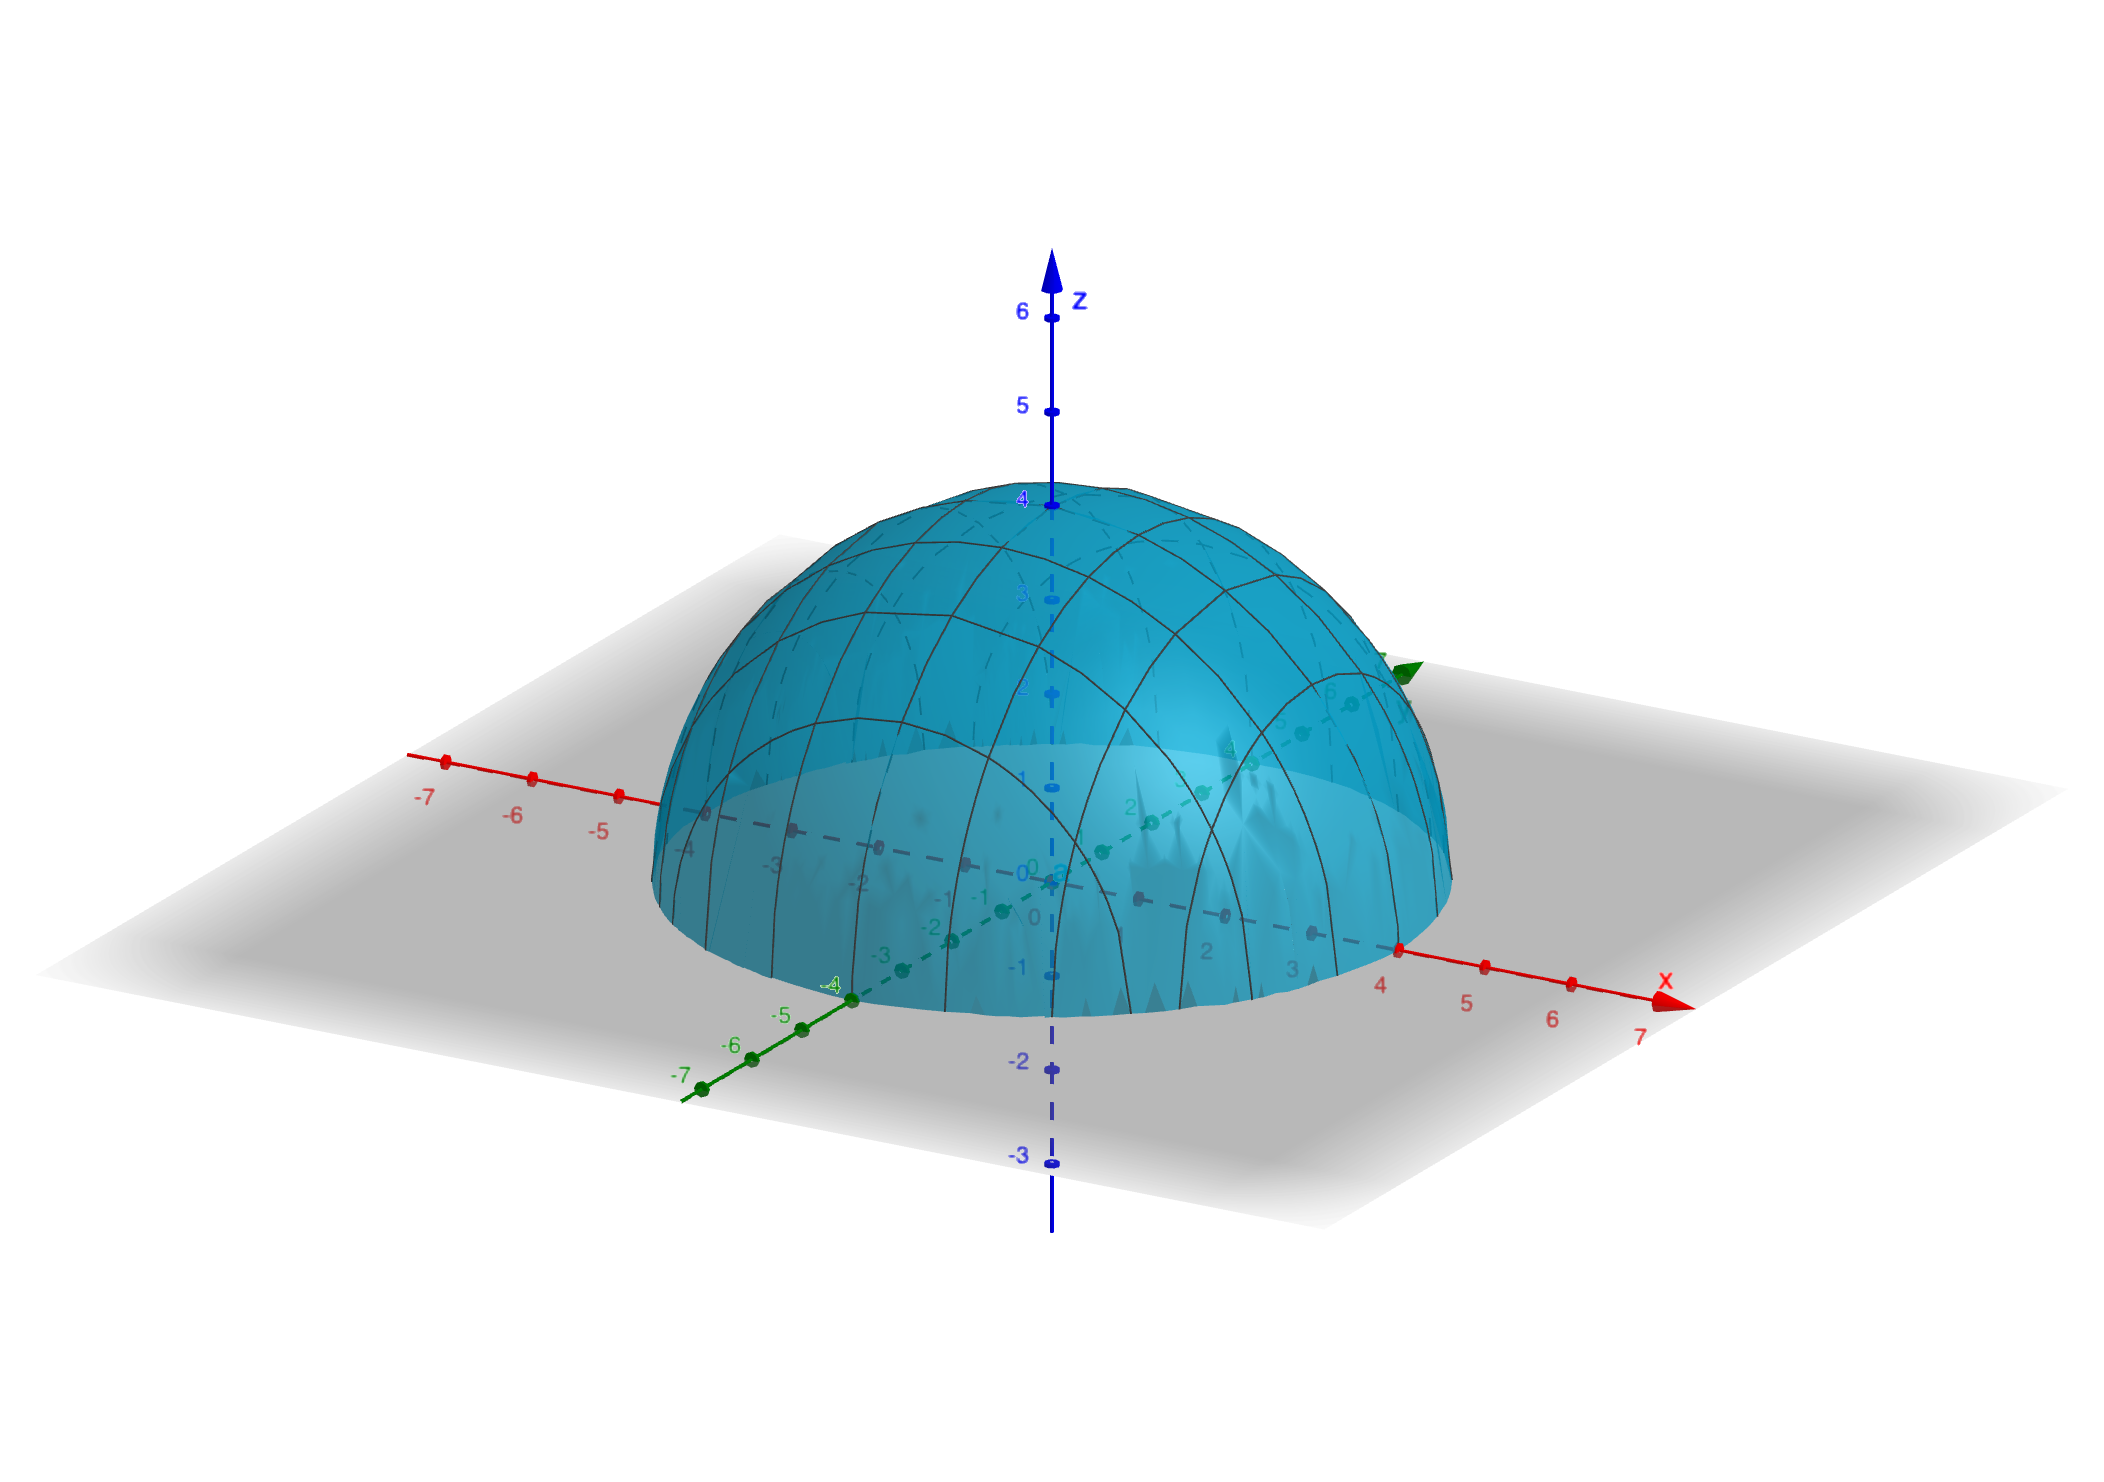
\includegraphics[scale=0.1]{images/11-ex1.png}    
\end{center}    
\end{proof}

\begin{definition} The contours of a function $f$ of two variables are the curves with equations $f(x,y) = k$, where $k$ is constant (in the range of $f$).
\end{definition}

\begin{example} Sketch the level curves of $f(x,y) = \frac{1}{x^2+y^2}$, with $k=\frac{1}{9}, \frac{1}{4}, 1, 4, 9$. Use these to attempt to sketch a 3D version of the graph.
\end{example}
\begin{proof} With $k=\frac{1}{3}$ we have $f(x,y) = \frac{1}{9}$ is equivalent to $x^2+y^2 = 3^2$, it is a cirlce. Similarly with $k=\frac{1}{4}$ it is a circle $x^2+y^2=4$. We have a set of cirles centered at $(0,0)$ with radius $3,2,1,\frac{1}{2}, \frac{1}{3}$, correspondingly to $k=\frac{1}{9}, \frac{1}{4}, 1, 4, 9$.
\clearpage
\begin{center}
    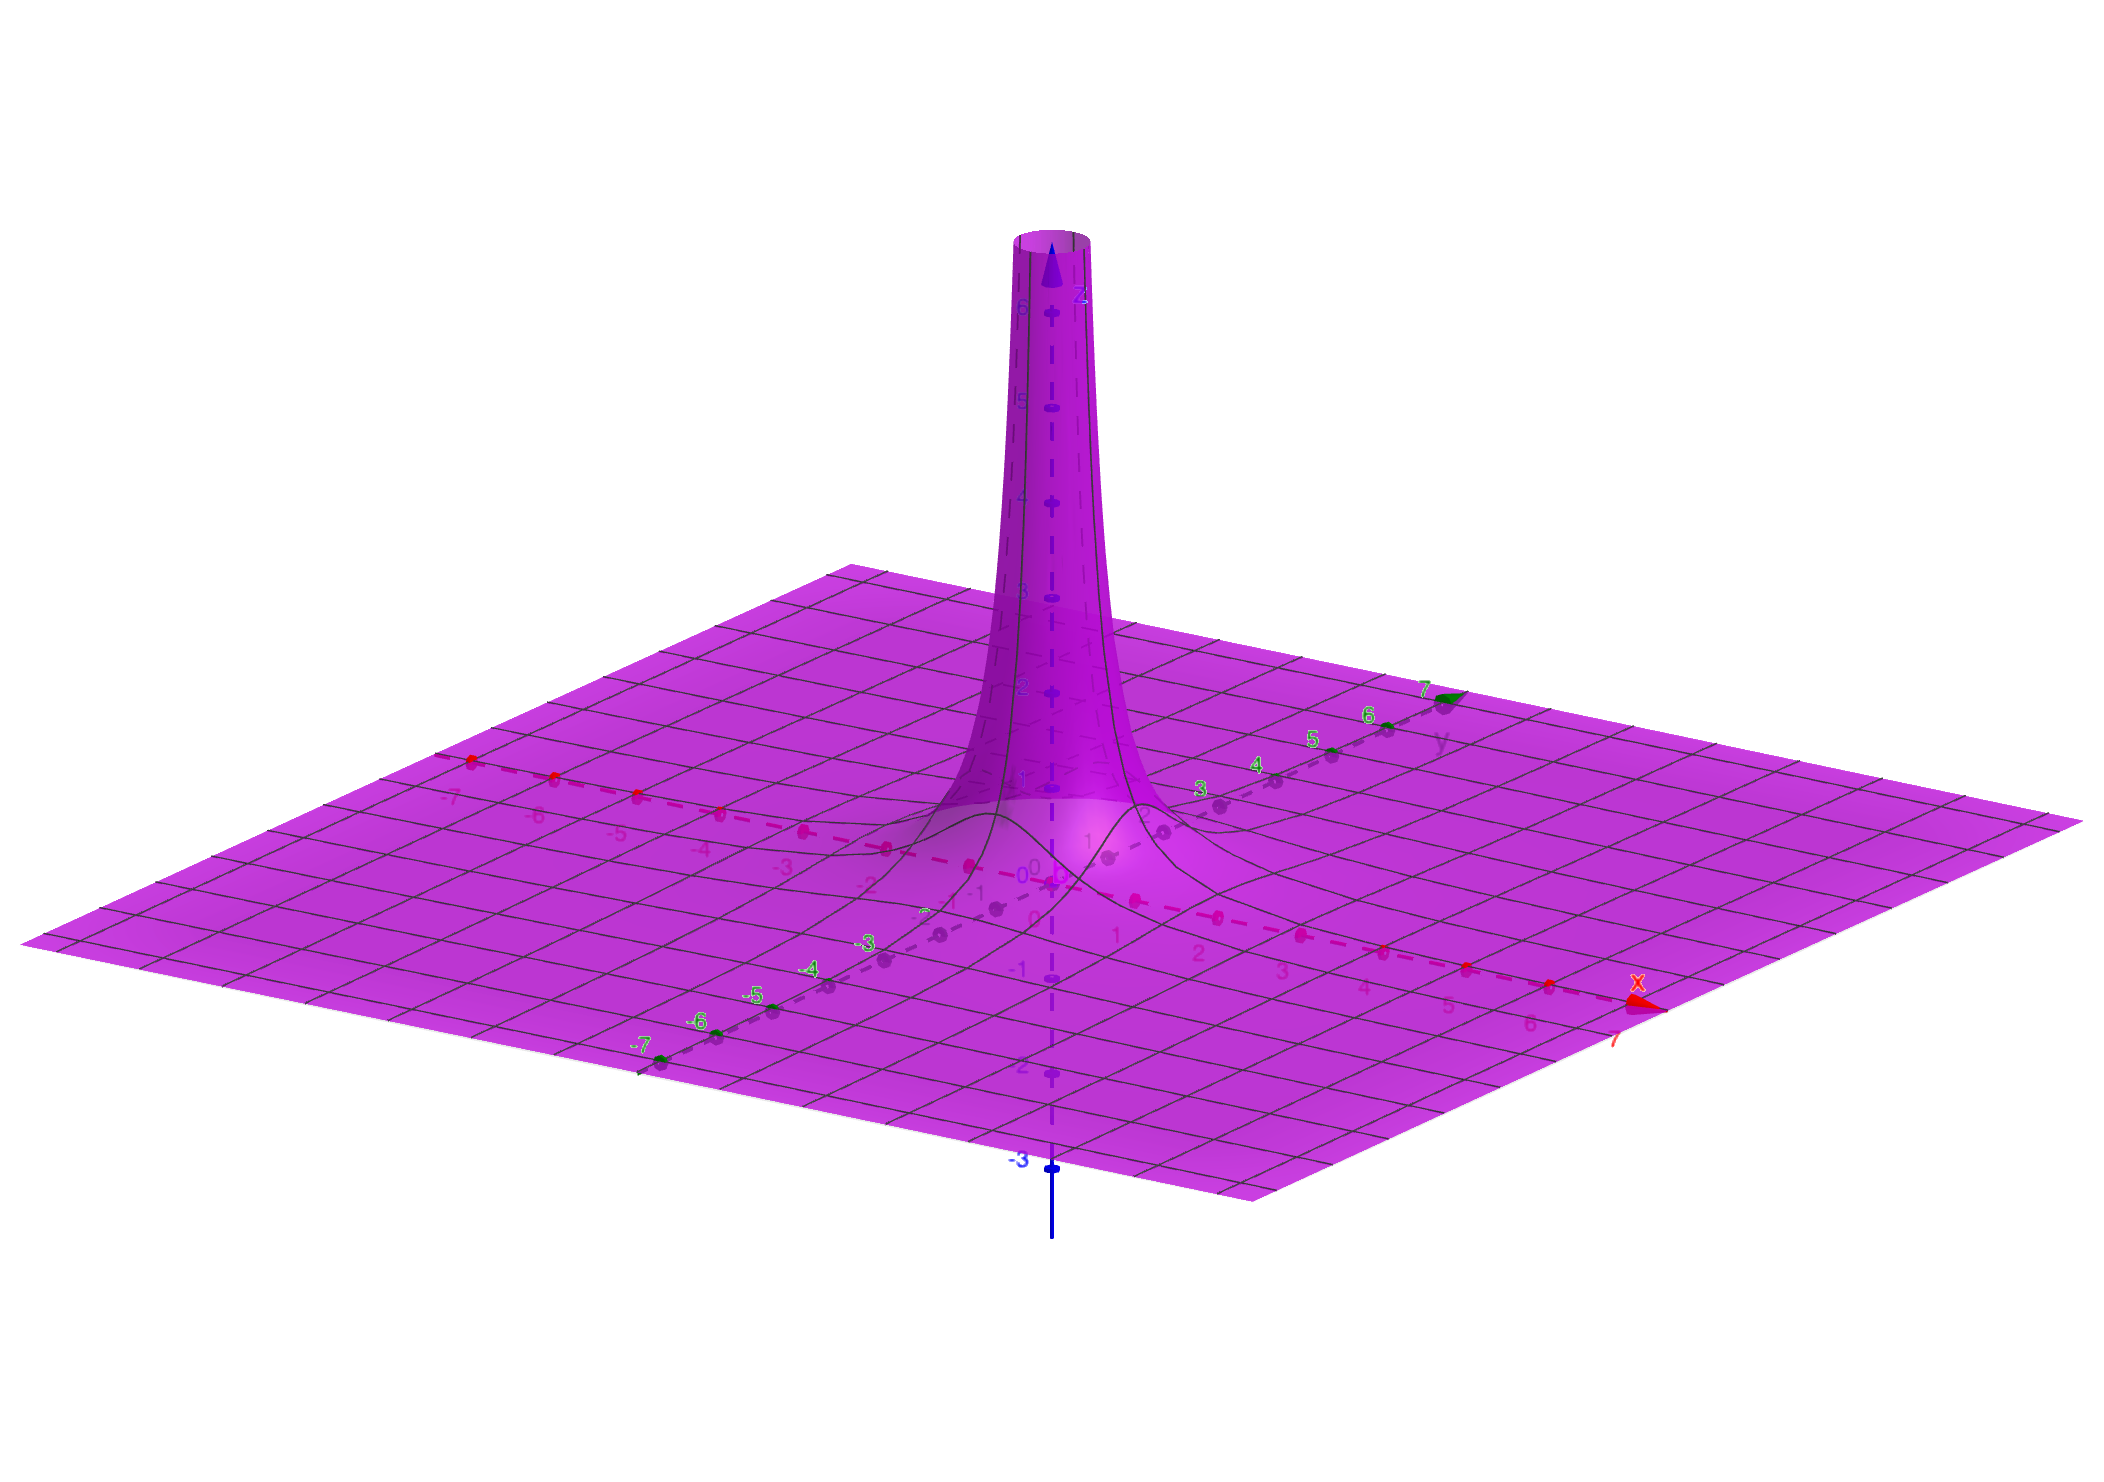
\includegraphics[scale=0.1]{images/11-ex2-a.png} \quad 
    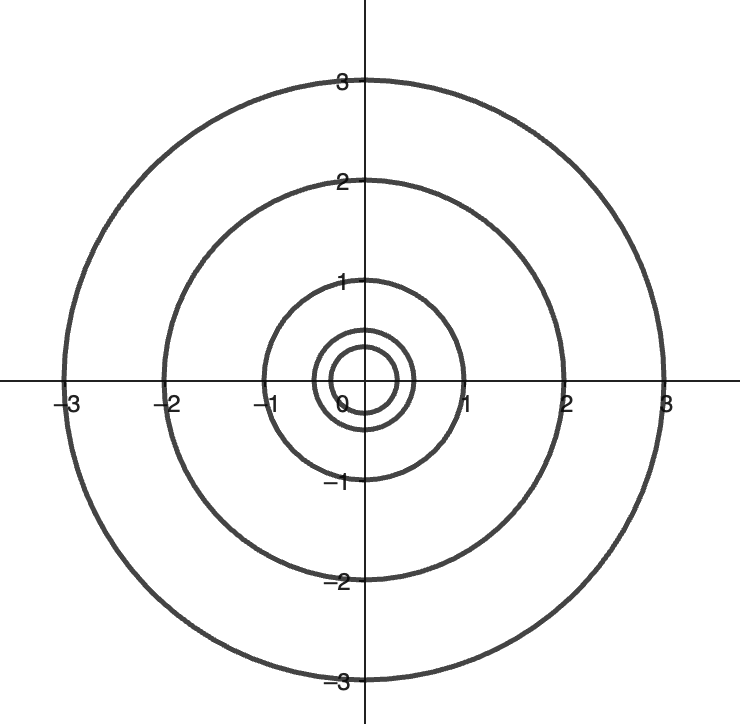
\includegraphics[scale=0.5]{images/11-ex2-b.png}    
\end{center}
Note: if $f(x,y)$ is a 2-variables function then $\mathrm{graph}(f)$ is 3D (on the left), but its contours are 2D as in the picture (on the right).
\end{proof}


\begin{definition} A function of 3 variables is $f(x,y,z)$ from a domain $D\subset \mathbb{R}^3$ to $\mathbb{R}$. The \textbf{level surfaces} of $f(x,y,z)$ are the surfaces with the equation $f(x,y,z) = k$ where $k$ is a constant (by looking at level surfaces, we can view it in 3D, instead of the graph of $f$ is in 4D).
\end{definition}

\begin{example} Find the domain of $f(x,y) = \frac{(x-1)(y+2)}{(y-x)(y-x^3)}$. Sketch and write the domain in set notation.
\end{example}
\begin{proof} $D=\{(x,y)\in \mathbb{R}^2: y\neq x, y\neq x^3\}$. The domain is the whole plane $\mathbb{R^2}$ (the $xy$-plane) removing the line $y=x$ and the curve $y=x^3$.

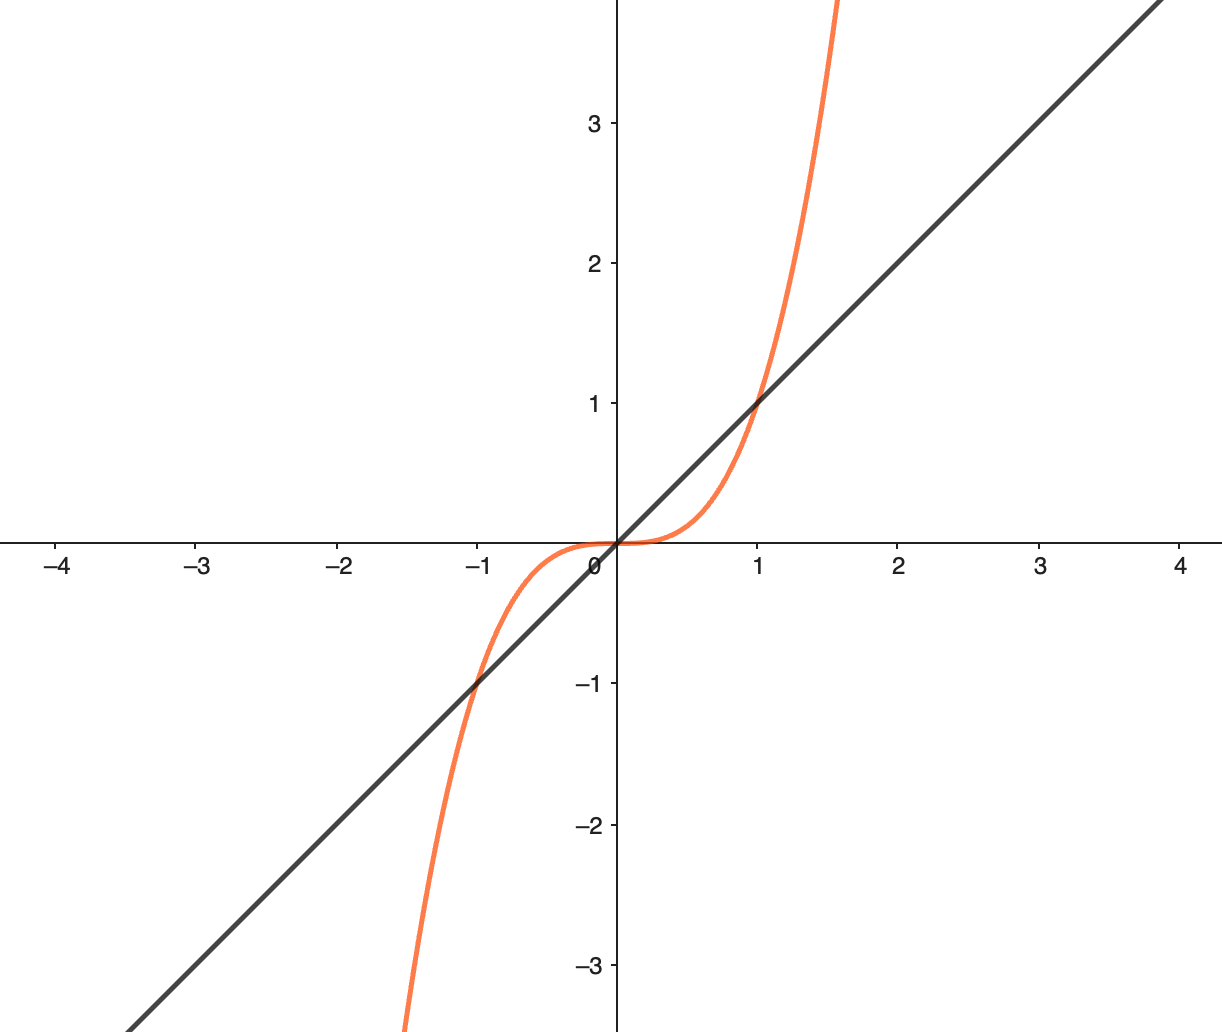
\includegraphics[scale=0.6]{images/11-ex3.png}    

\end{proof}

\begin{example} Consider the function $z=f(x,y) = \sqrt{y-x}$.
    \begin{itemize}
        \item[(a)] Dmain $D = \{(x,y): y-x\geq 0\}=\{(x,y): y\geq x\}$. (The line $y=x$ is included.)
        \begin{center}
            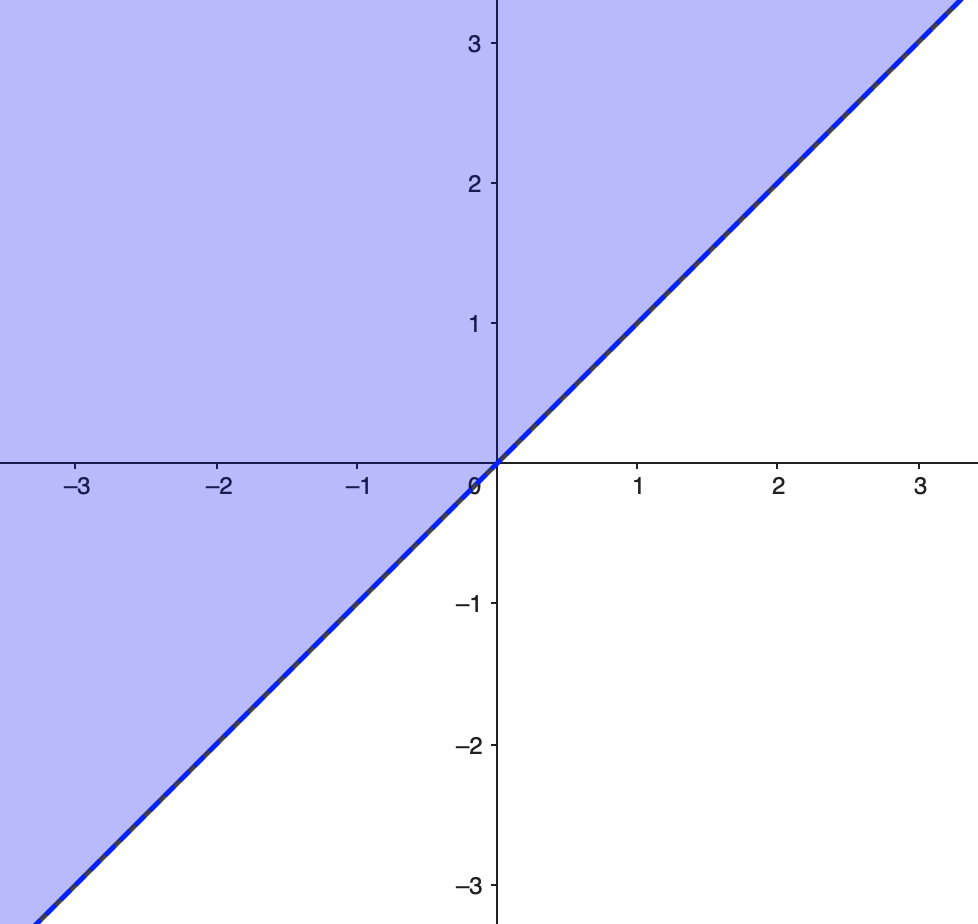
\includegraphics[scale=0.3]{images/11-ex4-a.png}
        \end{center}
        \item[(b)] The range is $z\in [0,+\infty)$.
        \item[(c)] Sketch some level curves and the graph
        \begin{center}
            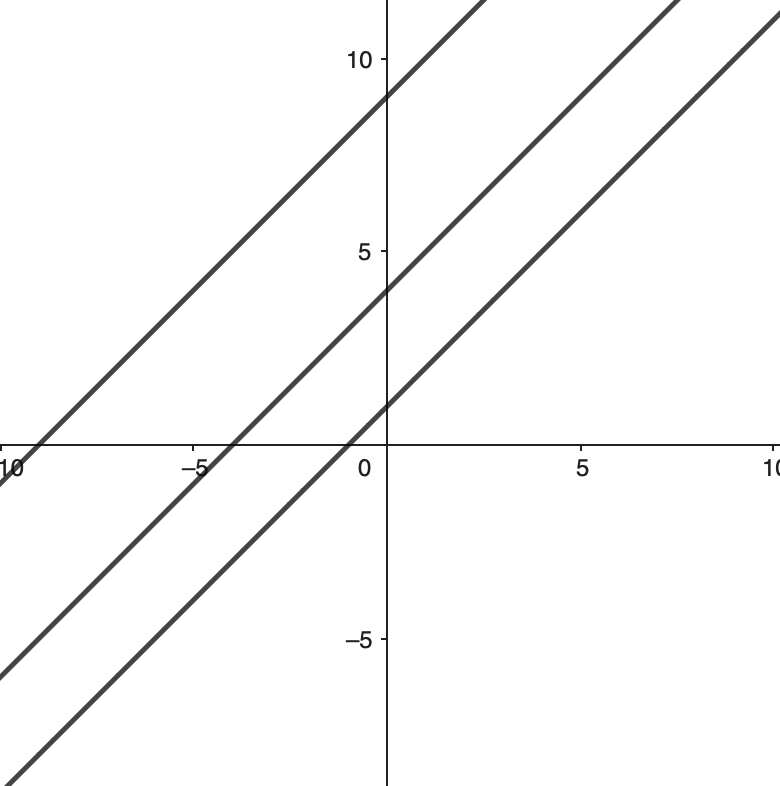
\includegraphics[scale=0.4]{images/11-ex4-b.png}\quad 
            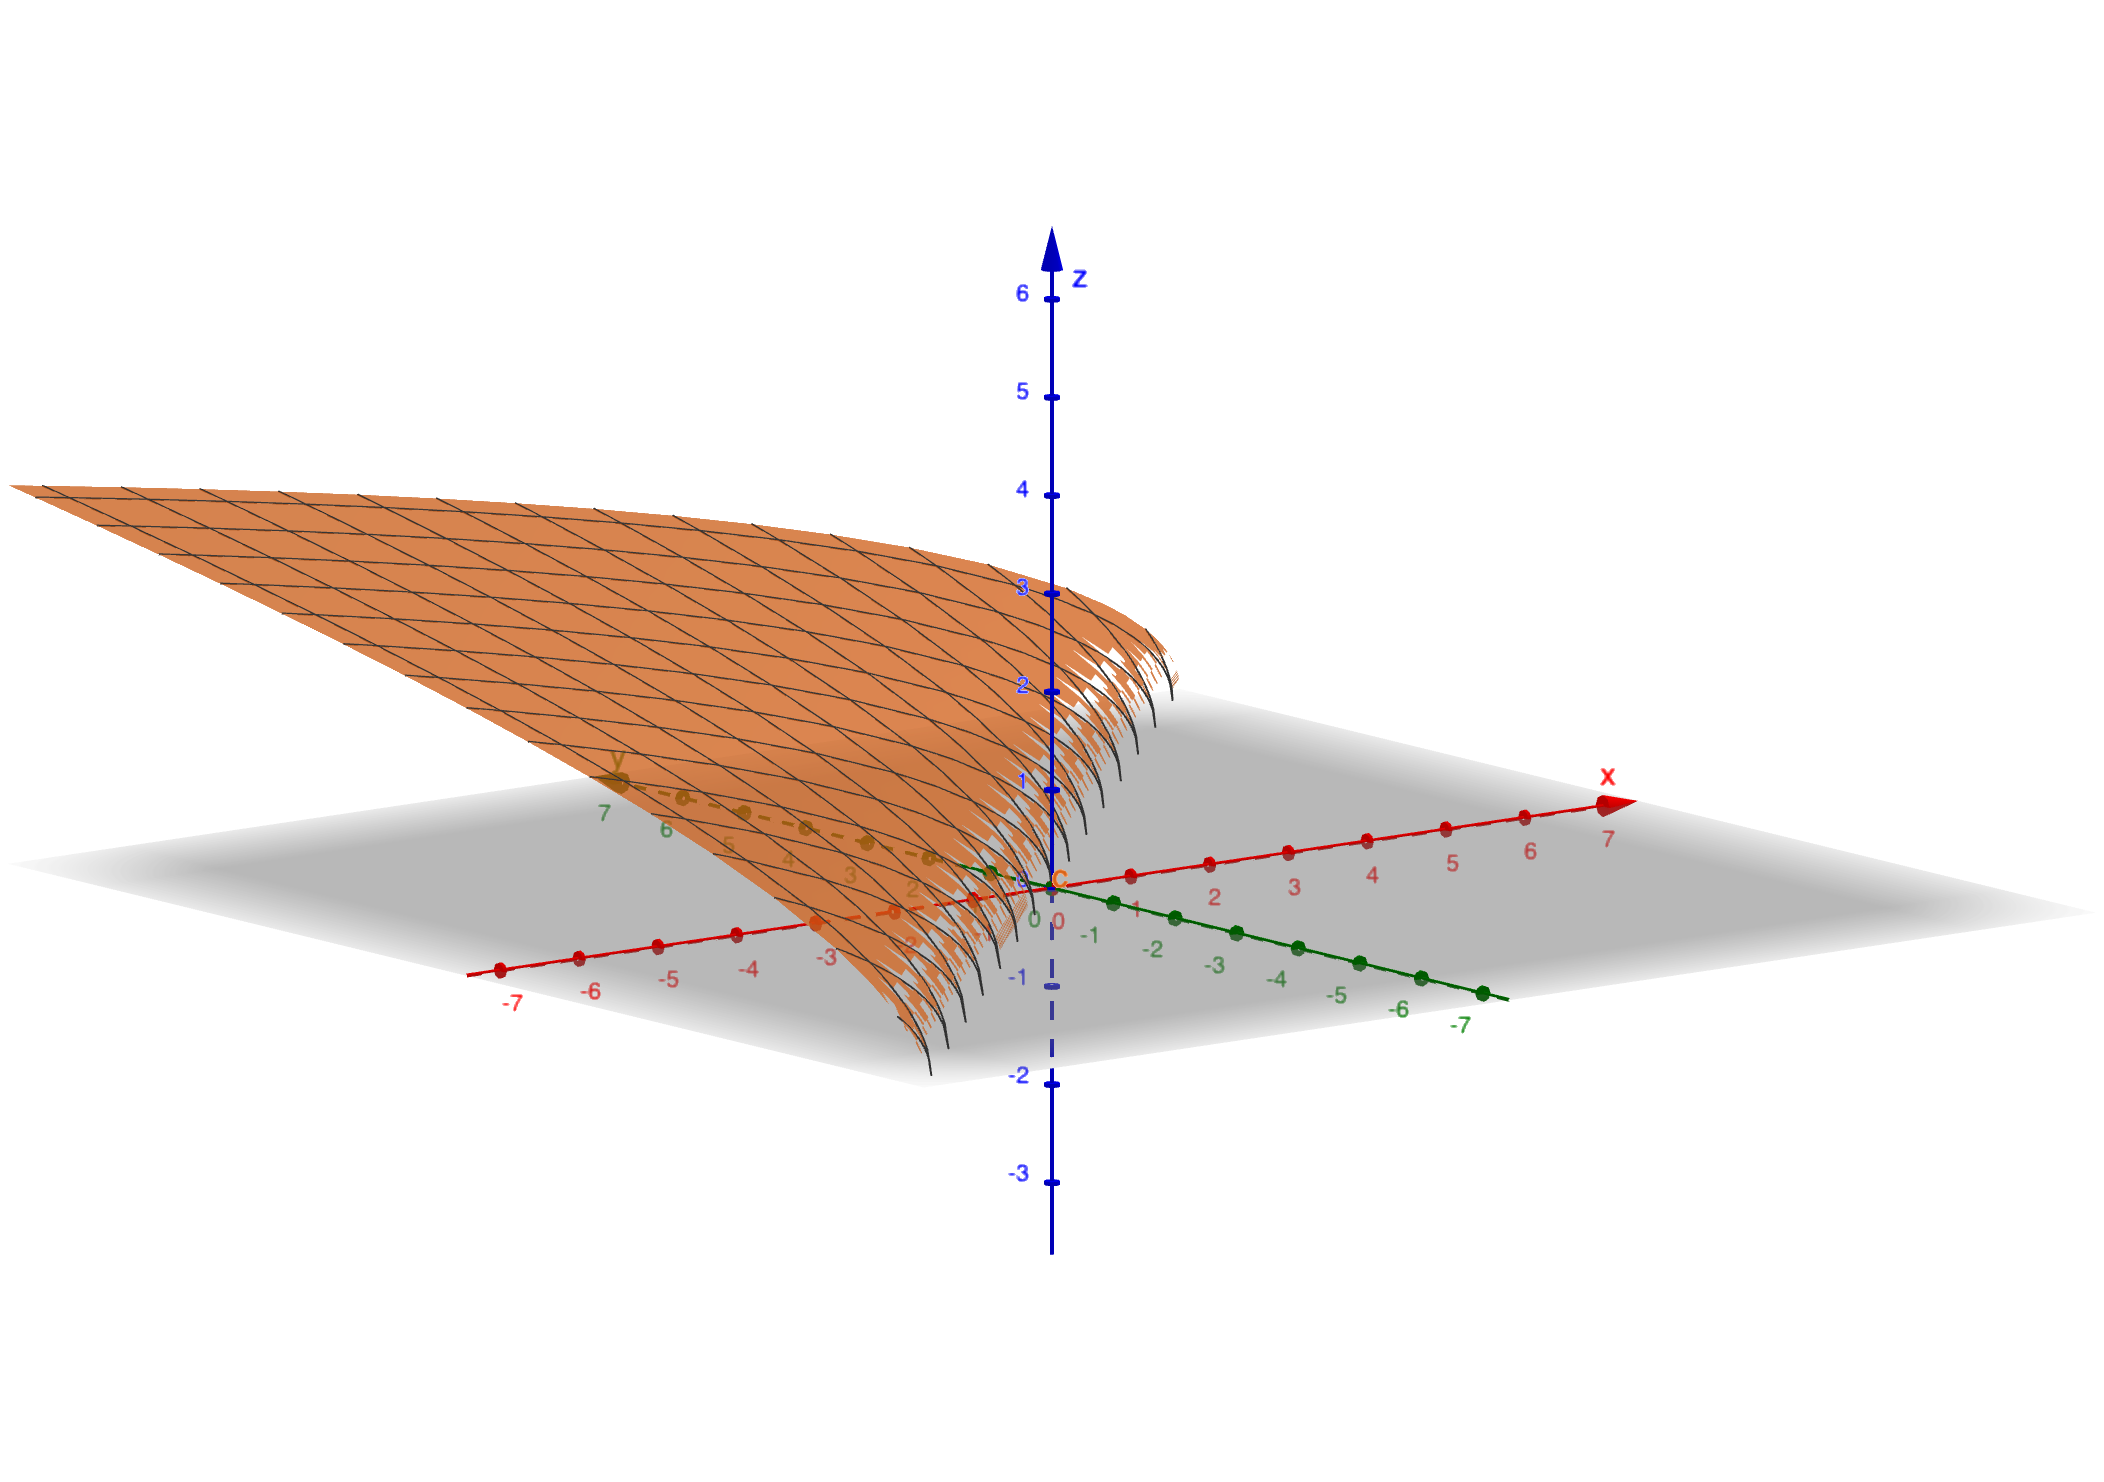
\includegraphics[scale=0.1]{images/11-ex4-c.png}
        \end{center}
    \end{itemize}
\end{example}


\section{Partial derivatives}

\begin{definition}[Partial Derivatives]\quad 
    \begin{itemize}
        \item[(a)] The partial derivatives of $f(x,y)$ with respect to $x$ at $(a,b)$ is denoted by $f_x(a,b)$ and is given by
        \begin{equation*}
            f_x(a,b) = \lim_{h\to 0} \frac{f(a+h,b) - f(a,b)}{|h|}. 
        \end{equation*}
        This is equivalent to considering $y$ as a constant and taking derivative in $x$.
        \item[(b)] The partial derivatives of $f(x,y)$ with respect to $y$ at $(a,b)$ is denoted by $f_y(a,b)$ and is given by
        \begin{equation*}
            f_y(a,b) = \lim_{k\to 0} \frac{f(a,b+k) - f(a,b)}{|k|}. 
        \end{equation*}
        This is equivalent to considering $x$ as a constant and taking derivative in $y$.
        \item[(c)] Other notations
        \begin{align*}
            f_x(x,y) &= f_x = \frac{\partial f}{\partial x} = \frac{\partial f}{\partial x}(x,y) = \frac{\partial z}{\partial x} = D_xf \\
            f_y(x,y) &= f_y = \frac{\partial f}{\partial y} = \frac{\partial f}{\partial y}(x,y) = \frac{\partial z}{\partial y} = D_yf .
        \end{align*}
        \item[(d)] Second-order derivatives:
        \begin{align*}
            (f_x)_x &= f_{xx} = \frac{\partial }{\partial x}\left(\frac{\partial f}{\partial x}\right) = \frac{\partial^2 f}{\partial x^2} = \frac{\partial^2 z}{\partial x^2} \\
            (f_y)_y &= f_{yy} = \frac{\partial }{\partial y}\left(\frac{\partial f}{\partial y}\right) = \frac{\partial^2 f}{\partial y^2} = \frac{\partial^2 z}{\partial y^2} \\
            (f_x)_y &= f_{xy} = \frac{\partial }{\partial y}\left(\frac{\partial f}{\partial x}\right) = \frac{\partial^2 f}{\partial y \partial x} = \frac{\partial^2 z}{\partial y \partial x} \\
            (f_y)_x &= f_{yx} = \frac{\partial }{\partial x}\left(\frac{\partial f}{\partial y}\right) = \frac{\partial^2 f}{\partial x \partial y} = \frac{\partial^2 z}{\partial x \partial y} .
        \end{align*}
        Note the sequence: the first derivative is taken closest to the function.
        \item[(e)] (Clairaut's Theorem) The order of taking derivatives (around a point $(a,b)$) does not matter if the second order derivaties are continuous and defined around a point $(a,b)$. 
        \begin{equation*}
            \frac{\partial }{\partial x} \frac{\partial f}{\partial y}(a,b) = \frac{\partial }{\partial y} \frac{\partial f}{\partial x}(a,b).
        \end{equation*}
        \item[(f)] The gradient
        \begin{equation*}
            \nabla f(a,b) = \left(f_x(a,b), f_y(a,b)\right)
        \end{equation*}
        gives the direction in which the value of the function increases the fastest.
    \end{itemize}
\end{definition}
\begin{example} We have
    \begin{align*}
        &\frac{\partial}{\partial x} \left(\frac{\partial}{\partial y} \left(xy + x\sin y + \frac{y}{x}\right)\right) =  \frac{\partial}{\partial x} \left(x + x\cos y + \frac{1}{x}\right) = 1 + \cos y -\frac{1}{x^2}\\
        &\frac{\partial}{\partial y} \left(\frac{\partial}{\partial x} \left(xy + x\sin y + \frac{y}{x}\right)\right) =  \frac{\partial}{\partial y} \left(y + \sin y - \frac{y}{x^2}\right) = 1 + \cos y -\frac{1}{x^2}\\
    \end{align*}
\end{example}

\begin{example} Let $v(x,y) = \frac{xy}{x-y}$. Compute $v_x, v_{xx}, v_{xy}$.
\end{example}
\begin{proof} We use product rule or quotient rule, or any rule from Calculus 1 and 2:
\begin{align*}
    v_x = \frac{y(x-y) - xy}{(x-y)^2} = \frac{-y^2}{(x-y)^2}, \qquad v_{xx} = \frac{- (-y^2)2(x-y)}{(x-y)^4} = \frac{2y^2}{(x-y)^3}\\
    v_{xy} = \frac{-2y(x-y)^2 - (-y^2)2(x-y)}{(x-y)^4} = \frac{-2y+2y^2}{(x-y)^3}.
\end{align*}
\end{proof}

\begin{example} Find $f_{xyz}$ for $f(x,y,z)= xyz + (x^2+y^2) \frac{\sin^{-1}(x\sqrt{y})}{\tan(x)}$. 
\end{example}
\begin{proof} Note that $\frac{\partial}{\partial x}(\sin^{-1}(x)) = \frac{\partial}{\partial x}(\arcsin(x)) = \frac{1}{\sqrt{1-x^2}}$. We compute (product rule, then quotient rule)
\begin{align*}
    f_x = yz + 2x \frac{\partial }{\partial x} \left((x^2+y^2) \frac{\sin^{-1}(x\sqrt{y})}{\tan(x)}\right).
\end{align*}
Let us not computing the derivative of that term for now, for a reason we will see soon. Now we have
\begin{align*}
    f_{xy} = \frac{\partial}{\partial y} f_x 
    &= \frac{\partial}{\partial y} (yz) + \frac{\partial}{\partial y}\left[2x \frac{\partial }{\partial x} \left((x^2+y^2) \frac{\sin^{-1}(x\sqrt{y})}{\tan(x)}\right)\right] \\
    &= z + \frac{\partial}{\partial y}\left[2x \frac{\partial }{\partial x} \left((x^2+y^2) \frac{\sin^{-1}(x\sqrt{y})}{\tan(x)}\right)\right].
\end{align*}
Now we have
\begin{align*}
    f_{xyz} = 1 + \frac{\partial}{\partial z} \underbrace{\frac{\partial}{\partial y}\left[2x \frac{\partial }{\partial x} \left((x^2+y^2) \frac{\sin^{-1}(x\sqrt{y})}{\tan(x)}\right)\right]}_{\text{no $z$ involved, thus this term is}\;0 }.
\end{align*}
The intergral is zero, since there is no $z$ involved, and we treat $x,y$ as constants when taking $\frac{\partial}{\partial z}$.
\end{proof}

\begin{example} Suppose you are surrounded by bees given by the bee density function
\begin{equation*}
    B(x,y) = 100-x^2+y^2+3y \qquad \text{bees}/\text{unit}^2.
\end{equation*}
You are currently standing at $(1,1)$. Which of the four directions would be best to run in $\{\textbf{i},-\textbf{i}, \textbf{j}, -\textbf{j}\}$?
\end{example}
\begin{proof} We have
    \begin{align*}
        \nabla B(x,y) = (-2x, 2y+3) \qquad \Longrightarrow\qquad \nabla B(1,1) = (-2, 5).
    \end{align*}
    The best direction to run would be the opposite of $(-2,5)$, i.e, $\textbf{v} = (2,-5)$. Now among the 4 directions, we choose the one that is closest, i.e., taking the dot product to find the one with smallest angle, i.e., $\cos \theta$ the biggest:
    \begin{itemize}
        \item For $\textbf{i} = (1,0)$ then $(1,0)\cdot(2,-5) = 2$.
        \item For $-\textbf{i} = (-1,0)$ then $(-1,0)\cdot(2,-5) = -2$.
        \item For $\textbf{j} = (0,1)$ then $(0,1)\cdot(2,-5) = -5$.
        \item For $-\textbf{j} = (0,-1)$ then $(0,-1)\cdot(2,-5) = 5$.
    \end{itemize}
    Therefore we choose $-\textbf{j}$.
\end{proof}